\tikzstyle{end} = [circle, minimum size = 0.1cm, draw, inner sep = 0.1pt]
\tikzstyle{leaf} = [circle, minimum size = 0.6cm, draw, inner sep = 0.1pt, blue]
            
\tikzstyle{level 1}=[level distance = 1.5cm, sibling distance = 2cm]
\tikzstyle{level 2}=[sibling distance = 2cm]
\tikzstyle{level 3}=[sibling distance = 2cm]
    
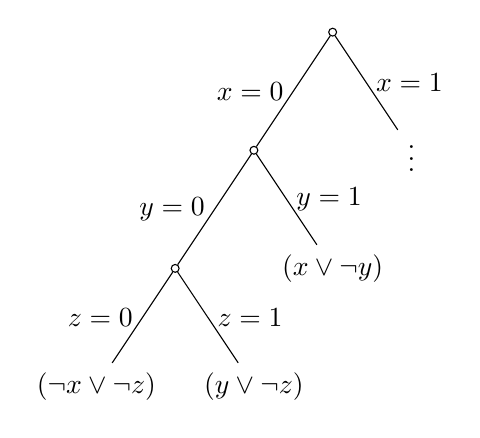
\begin{tikzpicture}[label distance=8mm]
	\node [end] (z){}
        child {
        	node[end] (b) {}
           	child {
               	node[end] {}
               	child {
                	node {\alert{$(\neg x \lor \neg z)$}}
	                edge from parent
		            node[left] {$z = 0$}
	            }
			    child {
	                node {\alert{$(y \lor \neg z)$}}
	                edge from parent
		            node[right] {$z = 1$}
	            }
                edge from parent
	            node[left] {$y = 0$}
            }
            child {
               	node {\alert{$(x \lor \neg y)$}}
                edge from parent
	            node[right] {$y = 1$}
            }
           	edge from parent
            node[left] {$x = 0$}
        }
        child {
        	node (b) {$\vdots$}
           	edge from parent
            node[right] {$x = 1$}
        };
\end{tikzpicture}

%%% Local Variables: 
%%% mode: latex
%%% TeX-master: t
%%% End: 
